\chapter{Planificación}
En este capítulo se recoge la planificación, el planteamiento y el principio de un proyecto al que hemos denominado ``\textbf{Fantasy}'', un portal web en el que los profesores pueden realizar una serie de tareas (fantasías) con el objetivo de que los alumnos puedan jugarlas y así aprendan de forma creativa.

Los alumnos, también tendrán la posibilidad de crear las fantasías que el profesor les mande como trabajo y luego serán evaluadas por dicho profesor.

\section{Metodología de desarrollo}
La metodología usada será \textbf{Scrum}: Método de desarrollo ágil caracterizado por tener un desarrollo incremental y basar la calidad del resultado en el conocimiento más que en los procesos empleados.

\section{Planificación del proyecto}
El proyecto tendrá una duración de tres meses y se realizarán reuniones semanales con el cliente de una hora de duración como máximo.
\begin{figure}[h]
	\centering
	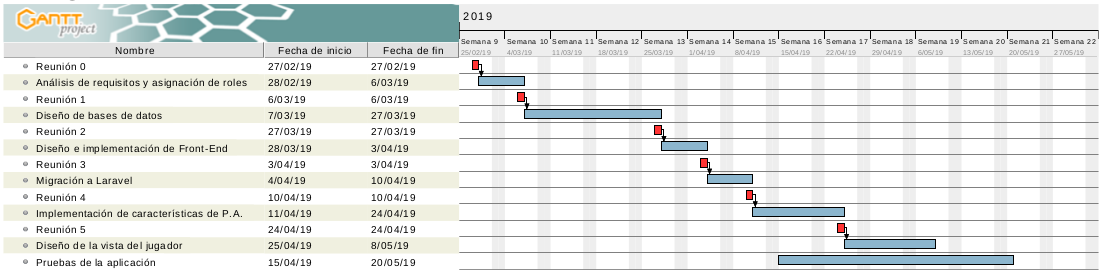
\includegraphics[scale=0.42]{Gantt.png}
	\caption{Diagrama de Gantt}
	\label{Diagrama de Gantt}
\end{figure}

\section{Organización}
\subsection{Roles}
\begin{itemize}
	\item \textbf{Administrador:} Luis Gutiérrez Flores.
	\item \textbf{Analistas:} Jesús Rodríguez Heras y Nicolás Ruiz Requejo.
	\item \textbf{Diseñadores:} Arantzazu Otal Alberro, Gabriel Fernando Sánchez Reina y Nicolás Ruiz Requejo.
	\item \textbf{Desarrolladores:} Luis Gutiérrez Flores, Alejandro Segovia Gallardo y Alejandro José Caraballo García.
	\item \textbf{Ingenieros de pruebas:} Jesús Rodríguez Heras y Luis Gutiérrez Flores.
\end{itemize}

\subsection{Recursos hardware y software}
Como recursos hardware tenemos los portátiles de los 7 miembros del grupo y el servidor de Stimey.

Como recursos software tenemos el framework Laravel, Atom, Visual Studio Code, TeXStudio, PhPMyAdmin, MySQL, GitHub.

\section{Costes}
\subsection{Costes humanos}
\begin{itemize}
	\item Horas en el aprendizaje de Laravel.
	\item Horas en formación de PHP y MySQL.
	\item Horas en formación de GitHub.
	\item Horas de documentación.
\end{itemize}

\subsection{Costes materiales}
\begin{itemize}
	\item Nuestros ordenadores.
	\item Transporte a la escuela.
	\item Gastos del servidor de Stimey.
\end{itemize}

\section{Gestión de riesgos}
\begin{itemize}
	\item No cumplir plazos por intentar abarcar demasiado y dejar funcionalidades incompletas.
\end{itemize}

\section{Política de equipo}
El equipo ha decidido hacer reuniones con una periodicidad de una semana con el cliente, a lo largo de la semana, los integrantes del equipo intentarán establecer reuniones entre ellos con la duración necesaria para continuar avanzando en el proyecto (tiempo estimado: dos horas).

\section{Hitos} %Seguir poniendo los demás sprints
\subsection{Sprint 0 (27 de febrero al 6 de marzo)}
\begin{enumerate}
	\item Creación de plataformas de trabajo y control de versiones (GitHub).
	\item Creación del boceto de requisitos.
	\item Creación de casos de uso y sus descripciones.
\end{enumerate}
\subsection{Sprint 1 (6 de marzo al 27 de marzo)}
\begin{enumerate}
	\item Creación de mockups de la plataforma.
	\item Implementación de la base de datos.
\end{enumerate}

\subsection{Sprint 2 (27 de marzo al 3 de abril)}
\begin{enumerate}
	\item Implementación de front-end.
	\item Migraciones de la base de datos.
	\item Adaptación del proyecto al framework Laravel.
	\item Creación de fantasías.
\end{enumerate}

\subsection{Sprint 3 (3 de abril al 10 de abril)}
\begin{enumerate}
	\item Finalización de front-end.
	\item Migraciones finales de la base de datos.
	\item Finalización de la creación de fantasías.
\end{enumerate}

\subsection{Sprint 4 (10 de abril al 24 de abril)}
\begin{enumerate}
	\item Finalización de las migraciones de la base de datos.
	\item Creación de puntos activos con sus características básicas.
\end{enumerate}

\subsection{Sprint 5 (24 de abril al 1 de mayo)}
\begin{enumerate}
	\item Creación de puntos activos con todas sus características.
	\item Inicio de la vista para poder jugar la fantasía.
\end{enumerate}


\section{Reuniones}
\subsection{Reunión 0 (27 de febrero)}
\begin{enumerate}
	\item Análisis de requisitos del sistema.
	\item Creación de casos de uso.
	\item Planteamiento de la base de datos del sistema.
	\item Distribución de las tareas del sprint 0.
\end{enumerate}

\subsection{Reunión 1 (6 de marzo)}
\begin{enumerate}
	\item Finalización del sprint 0.
	\item Distribución de la información a buscar.
	\item Comienzo del sprint 1.
\end{enumerate}

\subsection{Reunión 2 (27 de marzo)}
\begin{enumerate}
	\item Finalización del sprint 1.
	\item Comienzo del sprint 2.
\end{enumerate}

\subsection{Reunión 3 (3 de abril)}
\begin{enumerate}
	\item Finalización del sprint 2.
	\item Comienzo del sprint 3.
\end{enumerate}

\subsection{Reunión 4 (10 de abril)}
\begin{enumerate}
	\item Finalización del sprint 3.
	\item Comienzo del sprint 4.
\end{enumerate}

\subsection{Reunión 5 (24 de abril)}
\begin{enumerate}
	\item Finalización del sprint 4.
	\item Comienzo del sprint 5.
\end{enumerate}
